\section{Methodology}
\label{sec:model}

Figure~\ref{fig:modeloverview} illustrates the entire process of the GMH model. The input involves the head entity and relation of the incomplete triple with the background KG. The output is the missing tail entity.
We systematize the model in three steps:~1)~the local-global knowledge fusion module to integrate knowledge of history paths and graph structure;~2)~the differentiated action dropout module to diversify the reasoning paths; and~3)~the adaptive stopping search module to formulate the optimal steps of searching.
% The local-global factors fusion module fuses the local path and global embedding factors to facilitate the agent to select the positive path.
% The differentiated path dropout module forces the agent to explore a diverse set of paths from a global perspective.
% The adaptive stopping search uses a self-loop controller to avoid over searching and resource wasting.
The local-global knowledge fusion and differentiated action dropout modules facilitate the agent to address the issue of \textit{where to go}. The adaptive stopping search module controls the search steps to resolve the issue of \textit{when to stop}.

\subsection{Preliminary}
% \subsubsection{Definition}

% Before going to the detailed model description, 
We formally represent a KG as a collection of triples~$\mathcal{T}=\left \{ (e_{h},r,e_{t})|e_{h}\in \mathcal{E}, e_{t}\in \mathcal{E},r\in \mathcal{R}\right \} $, where $e_{h}$, $r$ and $e_{t}$ denote the head entity, relation and tail entity in one triple, $\mathcal{E}$ and $\mathcal{R}$ are the entity and relation sets, respectively. 
Each directed link in KG represents a valid triple~(i.e., $e_{h}$ and $e_{t}$ are represented as the nodes and $r$ as the labeled edge between them).
For an incomplete triple, multi-hop reasoning can be perceived as searching a target tail entity~$e_{t}$ through limited steps in KG, starting from head entity $e_{h}$ and based on the relation $r\in \mathcal{R}$. 
We use query~$q$ to represent $(e_{h},r)$ in the following sections.
At step $s$, the search agent will transfer to the entity~$e_{s}$ updating 
the history path trajectory~$\mathcal{H}_{s}=\left \{e_{h}, r_{1}, e_{1},..., r_{s}, e_{s}\right \}$, and the available action set  $\mathcal{A}_{s}=\left \{ ({{r_{s}^{i}}},{{e_{s}^{i}}} )|({e}_{s},{{r_{s}^{i}}},{{e_{s}^{i}}} )\in \mathcal{T}\right \}$.
%from which the agent will select one in the subsequent step. 
$\mathcal{A}_{s}$ consists of all outgoing relations and the associated entities of~${e}_{s}$.
The agent will select one action from~$\mathcal{A}_{s}$ to transfer to the next entity~${e}_{s+1}$ through the correlated relation~${r}_{s+1}$ at next step.  




\subsection{Local-Global Knowledge Fusion}

% \noindent
% \textbf{Fusing Local Path and global knowledges}
% \label{sec:Combine_his_tem}
In this module, we learn local knowledge~$lk_{s}$ and global knowledge~$gk_{s}$ to resolve the ``where to go" issue,
% assist the agent in effectively finding the target tail entity, 
as shown in Figure~\ref{fig:fusion}.
The local knowledge indicates that the agent makes decisions on the basis of the history path trajectory~$\mathcal{H}_{s}$ at step $s$ from a local perspective. 
The global knowledge is calculated through a pre-trained embedding-based models from a global perspective.
We use an aggregate~(abbr. AGG) block to aggregate $lk_{s}$ and $gk_{s}$, which has two types: summation~($lk_{s}+gk_{s}$) and scalar product~($lk_{s}*gk_{s}$).
The distribution $p(\mathcal{A}_{s})\in \mathbb{R}^{\left | \mathcal{A}_{s} \right |}$ is calculated through the AGG block and represents the confidence score for each available entity in $\mathcal{A}_{s}$.
% , and it lies on simplex of size $\left | \mathcal{A}_{s} \right |$.
The agent will select one action from~$\mathcal{A}_{s}$ according to the distribution $p(\mathcal{A}_{s})$
to transfer to the next entity.



\noindent
\textbf{Local Knowledge Learning}
% \label{sec:HTF}



The local knowledge~$lk_{s}$ indicates  from a local perspective that the agent makes decisions based on the history path trajectory~$\mathcal{H}_{s}$ at step $s$. We adopt long short-term memory~(LSTM) neural network and attention mechanism  to encode the history path trajectory and yield the local knowledge. 
% We expect that $lk_{s}$ contributes to improving the accuracy of the agent's decisions. 

The history path trajectory~$\mathcal{H}_{s}=(e_{h}, r_{1}, e_{1},..., r_{s}, e_{s})$ consists of the sequence of entities and relations which the agent has selected over the last $s$ steps. 
%Every entity and relation in $\mathcal{G}$ are assigned dense vector embeddings ${v_{e}}\in \mathbb{R}^{dim}$ and ${v_{r}}\in \mathbb{R}^{dim}$ by a look-up operation, where $dim$ is the dimension.
We adopt an embedding layer to generate the embedding of entities and relations.
The embedding of query is~$\vec{q}=[\vec{e_{h}};\vec{r}] \in \mathbb{R}^{2dim}$, i.e., the concatenation of the embeddings of the head entity $\vec{e_{h}}\in \mathbb{R}^{dim}$ and relation $\vec{r}\in \mathbb{R}^{dim}$, where $dim$ is the dimension.
We use an LSTM to encode the embedding of $\mathcal{H}_{s}$ to yield the hidden state embedding sequence $(\vec{h}_{0},...,\vec{h}_{s})$, where~$\vec{h}_{s}=LSTM(\vec{h}_{s-1},[{\vec{r_{s}}},{\vec{e_{s}}}])\in \mathbb{R}^{2dim}$ is the hidden state at step $s$,  ${e_{s}}$ is the current entity and ${r_{s}}$ is the relation that connects ${e_{s-1}}$ and ${e_{s}}$.


\begin{figure}[t]
        \setlength{\abovecaptionskip}{0.cm}
                \setlength{\belowcaptionskip}{-0.1cm}
\centering
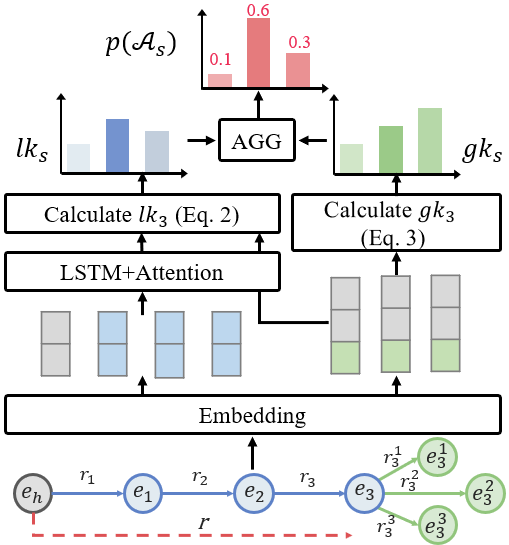
\includegraphics [width=0.39\textwidth]
{images//long_short2.png}
\caption{An illustration of the local-global knowledge fusion module. We reuse the search process in Figure 2 for detailed explanation. Best viewed in color.
% The left part learns the local knowledge
% from 
% % through encoding 
% the history path trajectory. 
% The right part learns the global knowledge from graph structure through a pre-trained embedding-base model. The fusion is conducted in the middle part and produces the probability distribution of
% % the final score for 
% the available actions.
% % Best viewed in color.
}
%\vspace{{-2mm}
\label{fig:fusion}      
\end{figure}

Prior works~\cite{das2017go,LinEMNLP2018} use only the current hidden state embedding~(i.e., $\vec{h}_{s}$) to yield the next action and they neglect the differentiated importance between the hidden states over the last $s$ steps.
Therefore, the attention weight value calculated between the hidden state embedding sequence and the query embedding is introduced to optimize the local knowledge~$lk_{s}$.
Each weight value is derived by comparing the query ${\vec{q}}$ with each hidden state~$\vec{h}_{i}$: 
\begin{equation}
\alpha({\vec{q}},\vec{h}_{i}) =\frac{\exp (f({\vec{q}},{\vec{h}_{i}}))}{\sum_{j=0}^{s}\exp (f({\vec{q}},{\vec{h}_{j}}))},
\end{equation}
where $i$ and $j$ stand for the $i$-th and $j$-th hidden state candidate, respectively.
Here, $f(\cdot )$ is represented as a query-based function: $f({v_{q}},{h_{m}})={v_{q}}^{\top }{h_{m}}$.
% \begin{equation}
% score({v_{q}},{h_{t}})={v_{q}}^{\top }{h_{t}}.
% \end{equation}
%The weight value reflects the internal correlation between the query $v_{q}$ and the history path trajectory $\mathcal{H}_{s}$. 
%The local knowledge~$lk_{s}$ reflects the influence of the history path trajectory on each element in the available action $\mathcal{A}_{s}$. 
Ultimately, local knowledge~$lk_{s} \in \mathbb{R}^{\left | \mathcal{A}_{s} \right |} $, which reflects the influence of the history path trajectory on each element in $\mathcal{A}_{s}$, can be obtained:
\begin{equation}
%HTF_{t}  =\sum_{t\in T}\alpha _{t}(r_{q})h_{t},
\vec{lk}_{s}  ={\mathcal{A}}_{s}\times {\bm{W}}_{1}\delta _{1}({\bm{W}}_{2}\sum_{m=1}^{s}\alpha({\vec{q}},\vec{h}_{m})\vec{h}_{m}),
\label{eq:lpf}
\end{equation}
\noindent where 
%${\mathcal{A}}_{t}$ is the available action set at step $s$, 
${\bm{W}}_{1}$ and ${\bm{W}}_{2}$ are the weights, and $\delta _{1}$ is the activation function.




\noindent
%\vspace{{-2mm}
\textbf{Global Knowledge Learning}
\label{sec:GEF}

Prior works~\cite{das2017go,LinEMNLP2018} use the local knowledge and neglect the long distance cases which requires higher decision accuracy of the agent.
We introduce the global knowledge~$gk_{s}$ learnt from graph structure by a pre-trained embedding-based model.
% adopt the existing embedding-based models to calculate the global knowledge~$gk_{s}$ from graph structure.

%The global knowledge~$gk_{s}$ indicates that the agent makes decisions on the basis of the query~$(e_{h},r_{q})$ from a global perspective by using existing embedding-based models.

Embedding-based models map the graph structure in continuous vector space by using a scoring function~$\psi(e_{h},r,e_{t})$.
% to maximize the score of each triple~$(e_{h},r,e_{t})$.
% learn global latent representations for entities and relations in continuous vector space and estimate the likelihood of each triple~$(e_{h},r,e_{t})$ by using a scoring function~$\psi(e_{h},r,e_{t})$.
We generate the new triple~$(e_{h},r,e_{s}^i)$ by concatenating the head entity and relation with available entity $e_{s}^i \in {\mathcal{E}}_{t}^{\mathcal{A}}$, where ${\mathcal{E}}_{t}^{\mathcal{A}}\in \mathbb{R}^{\left | \mathcal{A}_{s} \right |\times dim}$ contains all available entities in $\mathcal{A}_{s}$.
As we consider that the positive available entity is closer to the target tail entity in vector space, combining the positive available entity in $\mathcal{A}_{s}$ with the query will get a higher score than that using negative available entities.
% Therefore, we generate the new triple~$(e_{h},r,e_{s}^i)$ by concatenating the head entity and relation with $e_{s}^i \in {\mathcal{E}}_{t}^{\mathcal{A}}$, where ${\mathcal{E}}_{t}^{\mathcal{A}}\in \mathbb{R}^{\left | \mathcal{A}_{s} \right |\times dim}$ contains all available entities in $\mathcal{A}_{s}$.
% We adopt an embedding layer to generate the embedding of each new triple.
Formally, we adopt a pre-trained embedding-based model
% scoring function~$\psi(\cdot)$ 
to calculate these new triples to obtain the global knowledge~$gk_{s}$:
%The difference with the local knowledge~$HTF_{t}$ is that the global knowledge~$TTF_{t}$ relies on the similarity between the available action with the query entity and the query relation in the continuous vector space.
%Formally, the global knowledge~$TTF_{t}$ is defined as follows:
\begin{equation}
        \vec{gk}_{s} =[\psi({\vec{e}_{h}},\vec{r},{\vec{e}_{s}}^{~1});...;\psi({\vec{e}_{h}},\vec{r},\vec{e}_{s}^{~\left | \mathcal{A}_{s} \right |})].
\label{eq:gef}
\end{equation}
% where $N_{A}$ is the number of the available actions. 

Concatenating each of new triples' scores gives the global knowledge~$gk_{s} \in \mathbb{R}^{\left | \mathcal{A}_{s} \right |}$. The selection of scoring function~$\psi(\cdot)$ is discussed in Section~\ref{sec:ablation}.








\subsection{Differentiated Action Dropout}
\label{sec:actiondropout}
In the multi-hop reasoning task, it is important to enforce effective exploration of a diverse set of paths and dilute the impact of negative paths.
\cite{LinEMNLP2018} forced the agent to explore a diverse set of paths using action dropout technique which randomly masks some available actions in $\mathcal{A}_{s}$, i.e., blocking some outgoing edges of the agent. 
% Yet, that approach cannot discriminate paths of different qualities.
However, in the case of reasoning over long distances, the number of paths is much greater than that in the short distance scenarios because the search space grows exponentially.
The random action dropout technique is inefficient because it cannot discriminate paths of different qualities.
We then propose the differentiated action dropout~(DAD) technique based on the global knowledge~$gk_{s}$ to mask available actions, 
%Because we consider 
since we believe that higher-scoring actions are more likely to exist in a high-quality path.
In particular,
%In contrast, we use the global embedding factor~$GEF_{t}$ as the probability which is related to per available action. 
the mask matrix~$M_t \in \mathbb{R}^{\left | \mathcal{A}_{s} \right |}$ is sampled from the Bernoulli distribution:
\begin{equation}
        \vec{M}_t \sim  Bernoulli(sigmoid(\vec{gk}_{s})).
\label{eq:dropout}
\end{equation}

The element in $M_t$ is binary, where 1 indicates the action is reserved and 0 indicates abandonment.
The fusion of local-global knowledge and differentiated action dropout modules helps the agent to tackle the key problem~\textit{where to go} jointly.

%\vspace{{-2mm}
\subsection{Adaptive Stopping Search}
\label{sec:earlystopping}
For the second key issue of~\textit{when to stop}, 
we devise the adaptive stopping search~(ASS) module inspired by the early stopping strategy~\cite{Prechelt97earlystopping} which is used to avoid overfitting when training a learner with an iterative method.
We add a self-loop action~$($\textit{self-loop}$,e_{s})$ to give the agent an option of not expanding from~$e_{s}$.
When the agent chooses the self-loop action for several times, we consider it means that the agent has found the target tail entity, thus it can choose to end early.


In this module, we devise a self-loop controller to avoid over searching and resource wasting.
The self-loop controller has a dual judgment mechanism based on the the maximum search step~$S$ and the maximum loop number~$N$.
When the search step reaches the maximum~$S$, or the agent selects the self-loop action for $N$ consecutive times, the search process will be stopped.
Using the ASS strategy improves our model's scalability on both short and long distances and effectively avoids wasting of resources caused by over-searching.

\begin{algorithm}[t]
        \footnotesize
        \caption{Training process of GMH}
        \label{algorithm:training}
        \LinesNumbered
        \KwIn{The training samples set~$\mathcal{D}_{train}$;
                        background KG~($\mathcal{T}$, $\mathcal{E}$, $\mathcal{R}$);
                        the maximum search step~$S$;
                        the maximum loop number~$N$;
                        the randomly initialized parameters $\theta$
                        }
      \KwOut{The optimized parameters~$\theta$}

      \Repeat  {model converged}
      {
        Sample a triple $(e_{h},r,e_{t})$ from $\mathcal{D}_{train}$;
      
      \textbf{Initialize}: $s=0$; $n=0$;
      $e_{s}=e_{h}$; $\mathcal{H}_{s}=\left \{e_{h}\right \}$; $\mathcal{A}_{s}=\left \{ ({{r_{s}^{i}}},{{e_{s}^{i}}} )|({e}_{h},{{r_{s}^{i}}},{{e_{s}^{i}}} )\in \mathcal{T}\right \}$; 
      
      \For {$s<S$ and {$n<N$}}
      {
        % Calculate the local and global knowledge~$lk_{s}$~(Eq.~\ref{eq:lpf}) and the global knowledge~$gk_{s}$~(Eq.~\ref{eq:gef});
        Calculate $lk_{s}$~(Eq.~\ref{eq:lpf}) and $gk_{s}$~(Eq.~\ref{eq:gef});

        %        \State Calculate the global knowledge~$gk_{s}$~(Eq.~\ref{eq:gef})
        Fuse $lk_{s}$ and $gk_{s}$ to yield the final score;

        Dropout actions from~$\mathcal{A}_{s}$~(Eq.~\ref{eq:dropout});
        %  based on the mask matrix~$M_s$
         

        Select the next entity~$e_{s+1}$ and the related relation~$r_{s+1}$;
        
        \If {$r_{s+1}=$self-loop}{             $n\leftarrow n+1$;
}
                
        \textbf{update} $His_{s+1}\leftarrow \mathcal{H}_{s}\cup \left \{r_{s+1},e_{s+1}\right \}$; $\mathcal{A}_{s+1}\leftarrow \left \{ ({{r_{s+1}^{i}}},{{e_{s+1}^{i}}} )|({e}_{s+1},{{r_{s+1}^{i}}},{{e_{s+1}^{i}}} )\in \mathcal{T}\right \}$;
        
        $s\leftarrow s+1$;
      }
      $\hat{e_{t}}=e_{s}$; calculate the reward~$R(\hat{e_{t}}|e_{h},r,e_{t})$ and update $\theta$~(Eq.~\ref{eq:gradient});
      }
\end{algorithm}

%\vspace{{-2mm}
\subsection{Training}
\label{sec:training}



Following~\cite{das2017go}, we frame the search process as a Markov Decision Process~(MDP) on the KG
%: on the basis of the query relation~$r_{q}$, the initial state is $e_{s}$ is updated to a new entity by the agent's decision at each step until the state arrives at the target entity~$e_{d}$.
and adopt the on-policy RL method to train the agent. 
We design a randomized history-dependent policy network $\pi=(p(\mathcal{A}_{1}),...,p(\mathcal{A}_{s}),...,p(\mathcal{A}_{S}))$.
The policy network is trained by maximizing the expected reward over all training samples~$\mathcal{D}_{train}$:
\begin{equation}
\begin{aligned}
J(\theta)=&\mathbb{E}_{(e_{h},r,e_{t})\sim \mathcal{D}_{train}}\\
&[\mathbb{E}_{A_{1},...,A_{S}\sim \pi}[R(\hat{e_{t}}|e_{h},r,e_{t})]].
\end{aligned}
%%%%%\vspace{{-2mm}
\end{equation}

where $\theta$ denotes the set of parameters in GMH, $R(\cdot )$ is the reward function and $\hat{e_{t}}$ is the final entity chosen by the agent. If $\hat{e_{t}}={e}_{t}$, then the terminal reward is assigned +1 and 0 otherwise.

The optimization is conducted using the REINFORCE algorithm~\cite{reinforce1994} which iterates through all $(e_{h},r,e_{t})$ triples in $\mathcal{D}_{train}$ and updates $\theta $ with the following stochastic gradient:%%%%%\vspace{{-3mm}
\begin{equation}
        \bigtriangledown _{\theta }J(\theta )\approx \bigtriangledown _{\theta }\sum\nolimits_{s}R(\hat{e_{t}}|e_{h},r,e_{t})\log \pi _{\theta }.
\label{eq:gradient}    
\end{equation}

The training process is detailed in Algorithm 1. 
% It takes as input the training samples set, background KG, the maximum search step, the maximum loop number and the randomly initialized parameters.
During a search process, 
% For each triple in the training samples set, GMH finds the tail entity based on the head entity and relation through traversing in the background KG.
for each search step, the agent takes three operations: local-global knowledge fusion~(lines 5-6), differentiated action dropout~(line 7) and adaptive stopping search~(lines 8-10).
After finding the tail entity, the reward is calculated and the parameters are updated~(line 13).
Finally, the optimized parameters are output.

%Our experiments are discussed in the next section.

